\documentclass[UTF8,aspectratio=169]{ctexbeamer}
\usetheme{Madrid}
\usecolortheme{default}
\usepackage{amsmath}
\usepackage{booktabs}
\usepackage{siunitx}
\usepackage{graphicx}
\usepackage{array}
\usepackage{xcolor}
\usepackage{xurl}
\usepackage{tikz}
\usetikzlibrary{positioning,arrows.meta,shapes.geometric}

\newcommand{\good}[1]{\textcolor{green!45!black}{#1}}
\newcommand{\warn}[1]{\textcolor{red!65!black}{#1}}
\newcommand{\bluenote}[1]{\textcolor{blue!65!black}{#1}}
\newcommand{\src}[1]{\vfill{\tiny\textcolor{gray!75!black}{Source: \url{#1}}}}
\newcolumntype{L}[1]{>{\raggedright\arraybackslash}p{#1}}
\newcolumntype{R}[1]{>{\raggedleft\arraybackslash}p{#1}}
\newcolumntype{C}[1]{>{\centering\arraybackslash}p{#1}}

\title[Three Derived Populations]{Three Derived Populations from the Cleaned Penetration Archive\\Structure, Role, and Thesis Update Plan}
\author{Mie Spray Postprocessing Project}
\date{\today}

\begin{document}

\begin{frame}
  \titlepage
\end{frame}

% ──────────────────────────────────────────────────────────────
\begin{frame}{Message}
\small
\textbf{Claim:} the cleaned penetration archive produced by \texttt{fit\_raw\_data.py} is read by the downstream pipeline through \warn{three structurally distinct data populations}, each with its own construction protocol, selection bias, and pipeline role. They are not interchangeable, and the current thesis section 4 conflates two of them.

\vspace{0.45em}
\textbf{What this deck does:}
\begin{itemize}
  \item name the three populations explicitly and tie each one to its on-disk artefact;
  \item map each population to the exact training/evaluation entry point that consumes it (code-verified, not narrative);
  \item flag the one place where the thesis narrative is currently ambiguous (Stage-1 ``representative trajectory'' vs.\ p50 oracle);
  \item record the concrete edits that section 4 needs.
\end{itemize}

\vspace{0.45em}
\textbf{Scope:} this is a structural planning deck. It does \emph{not} re-derive metrics or repeat the q1 scaling story --- it just reorganises what already exists so the thesis can cite it cleanly.
\end{frame}

% ──────────────────────────────────────────────────────────────
\begin{frame}{Where the Populations Live in the Pipeline}
\small
\begin{center}
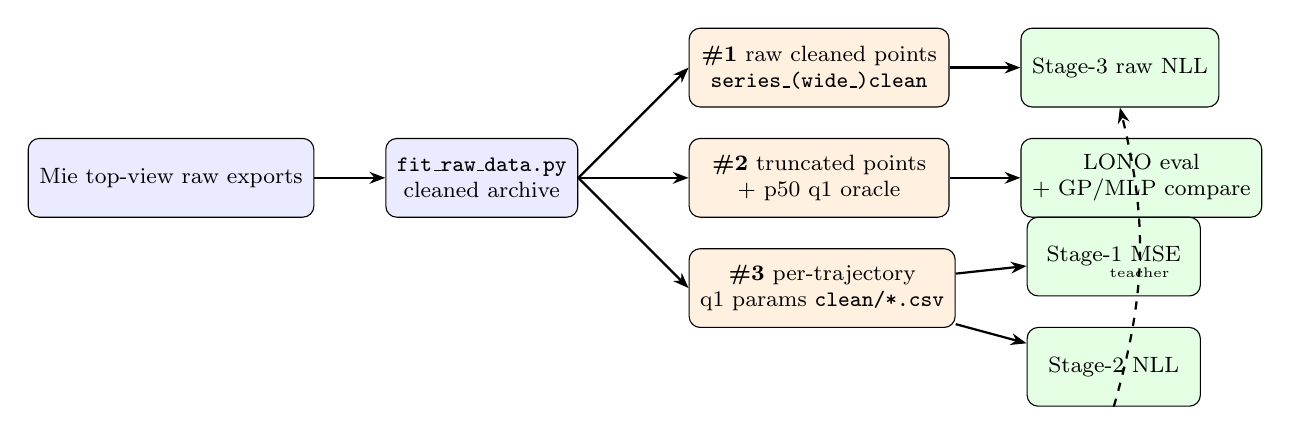
\begin{tikzpicture}[
  node distance=4mm and 9mm,
  every node/.style={font=\footnotesize},
  box/.style={draw, rounded corners, align=center, inner sep=4pt, minimum height=10mm},
  src/.style={box, fill=blue!8},
  pop/.style={box, fill=orange!12, minimum width=33mm},
  stage/.style={box, fill=green!10, minimum width=22mm},
  arrow/.style={-{Stealth[length=2mm]}, thick}
]
\node[src] (raw) {Mie top-view raw exports};
\node[src, right=of raw] (clean) {\texttt{fit\_raw\_data.py}\\cleaned archive};

\node[pop, right=14mm of clean, yshift=14mm] (d1) {\textbf{\#1} raw cleaned points\\\texttt{series\_(wide\_)clean}};
\node[pop, right=14mm of clean] (d2) {\textbf{\#2} truncated points\\+ p50 q1 oracle};
\node[pop, right=14mm of clean, yshift=-14mm] (d3) {\textbf{\#3} per-trajectory\\q1 params \texttt{clean/*.csv}};

\node[stage, right=of d1] (s3) {Stage-3 raw NLL};
\node[stage, right=of d2] (lono) {LONO eval\\+ GP/MLP compare};
\node[stage, right=of d3, yshift=4mm] (s1) {Stage-1 MSE};
\node[stage, right=of d3, yshift=-10mm] (s2) {Stage-2 NLL};

\draw[arrow] (raw) -- (clean);
\draw[arrow] (clean.east) -- (d1.west);
\draw[arrow] (clean.east) -- (d2.west);
\draw[arrow] (clean.east) -- (d3.west);

\draw[arrow] (d1) -- (s3);
\draw[arrow] (d2) -- (lono);
\draw[arrow] (d3) -- (s1);
\draw[arrow] (d3) -- (s2);
\draw[arrow, dashed] (s2.south) to[bend right=15] node[midway, below, font=\tiny]{teacher} (s3.south);
\end{tikzpicture}
\end{center}

\vspace{0.3em}
Three populations branch from the same cleaned archive, then re-converge only at Stage-3, where dataset \#1 supplies raw supervision and the Stage-2 teacher (trained on \#3) supplies the distillation prior. Dataset \#2 never enters training --- it is the external evaluation ruler.
\end{frame}

% ──────────────────────────────────────────────────────────────
\begin{frame}{Dataset \#1: Raw Cleaned Penetration (Discrete Observations)}
\small
\textbf{What it is.} The per-frame \((t, S)\) observations that survive cleaning, hydraulic-delay alignment, jump masks, and basic fit-quality gates. Two on-disk shapes:
\begin{itemize}\setlength\itemsep{1.5pt}
  \item long form: \path{MLP/synthetic_data/<nozzle>/cdf/series_clean/*.csv}
  \item wide form: \path{MLP/synthetic_data/<nozzle>/cdf/series_wide_clean/*.csv}
\end{itemize}

\vspace{0.35em}
\textbf{Size (clean archive).} \(\sim\)24{,}316 accepted trajectories, \(\sim\)703{,}592 individual frame observations.

\vspace{0.35em}
\textbf{Strengths.}
\begin{itemize}\setlength\itemsep{1.5pt}
  \item highest pointwise fidelity --- the closest thing to a measurement record;
  \item preserves the full per-frame heteroscedastic noise.
\end{itemize}

\textbf{Limitations.}
\begin{itemize}\setlength\itemsep{1.5pt}
  \item \warn{right-censored} (\(\sim 40\%\) of trajectories hit the FOV cap, per the audit in \S 4.1);
  \item non-uniform time sampling per condition --- late bins have few survivors.
\end{itemize}

\vspace{0.35em}
\textbf{Code entry point.} \texttt{load\_source\_table("cdf", split="clean")} in \path{train_stage3_distillation_plus_raw_series.py}, lines 241/247.

\textbf{Used by.} Stage-3 only --- as \good{direct raw supervision} in the \texttt{raw\_reliable} regime.
\end{frame}

% ──────────────────────────────────────────────────────────────
\begin{frame}{Dataset \#2: Statistically Cleaned Points + p50 q1 Oracle}
\small
\textbf{What it is.} Two artefacts derived by aggregating \#1 across trajectories within each operating condition:
\begin{enumerate}\setlength\itemsep{1pt}
  \item \textbf{uncensored point set} --- per-condition binning at \(\Delta t = \SI{0.1}{ms}\), then truncation at the first bin satisfying either: smoothed trajectory count below a fixed fraction of its within-condition peak (density-drop), or per-bin \(p_{95}\) penetration reaching \(95\%\) of the FOV cap (FOV-saturation);
  \item \textbf{p50 q1 oracle} --- per condition, take \(p_{50}\) of penetration in each surviving bin, fit q1 to the resulting \(\sim 5\)--\(45\) point trace.
\end{enumerate}

\vspace{0.35em}
\textbf{Size.} 506{,}634 uncensored points across 592 conditions; p50 oracle covers 495 conditions with median fit RMSE \SI{0.85}{mm}.

\vspace{0.35em}
\textbf{Strengths.}
\begin{itemize}\setlength\itemsep{1.5pt}
  \item \good{independent of the robust-z trajectory filter} used by Stage-2 \(\Rightarrow\) does not inherit the optical-quality + monotonicity selection bias of \#3;
  \item per-condition p50 absorbs plume-to-plume noise, giving a clean ceiling for what any condition-conditioned learner could achieve.
\end{itemize}

\textbf{Limitations.}
\begin{itemize}\setlength\itemsep{1.5pt}
  \item the density-drop and FOV-95\% thresholds are engineering choices, not data-derived;
  \item not a ground truth --- a \emph{less biased reference}, not an unbiased one.
\end{itemize}

\vspace{0.35em}
\textbf{Code entry.} \path{cdf_points_uncensored.csv} + \path{p50_q1_fit_metrics.csv} consumed by \texttt{eval\_on\_uncensored\_points} and \texttt{oracle\_metrics\_for\_holdout} in \path{run_lono_pipeline.py} (lines 216, 286).

\textbf{Used by.} \good{LONO out-of-distribution evaluation} and the GP vs.\ MLP cross-architecture comparison. \warn{Never enters training.}
\end{frame}

% ──────────────────────────────────────────────────────────────
\begin{frame}{Dataset \#3: Per-Trajectory q1 Parameter Set}
\small
\textbf{What it is.} For each accepted plume trajectory, the three q1 parameters \((\log k_{1/4}, \log t_0, \log s)\) fitted by Huber-NLLS to that trajectory's own \((t, S)\) observations. One CSV per cleaned dataset under \path{MLP/synthetic_data/<nozzle>/cdf/clean/*.csv}.

\vspace{0.4em}
\textbf{Size.} 24{,}316 accepted trajectories (clean-fit archive).

\vspace{0.4em}
\textbf{Strengths.}
\begin{itemize}\setlength\itemsep{1.5pt}
  \item smooth, differentiable, extrapolable to \SI{5}{ms} via the \(t^{1/4}\) prior;
  \item preserves between-trajectory variance required for the Stage-2 heteroscedastic NLL;
  \item compresses each long trajectory to three numbers \(\Rightarrow\) trainable with a small MLP on a master's compute budget.
\end{itemize}

\textbf{Limitations.}
\begin{itemize}\setlength\itemsep{1.5pt}
  \item \warn{inherits the robust-z selection bias} (optical quality + monotonicity);
  \item parameters are soft-coupled (median \(\operatorname{corr}(\log k_{1/4}, \log s) \approx 0.76\)) --- the three components are not independent physical handles.
\end{itemize}

\vspace{0.4em}
\textbf{Code entry.} \texttt{iter\_clean\_csv\_files} + \texttt{select\_representative\_row} (Stage-1) / \texttt{select\_filtered\_rows} (Stage-2) in \path{engineered_feature_common.py}, lines 480/503/529.

\textbf{Used by.}
\begin{itemize}\setlength\itemsep{1pt}
  \item \textbf{Stage-1 (599 trajectories)} --- \texttt{selection\_mode="representative"}: per condition group, pick the single trajectory whose q1-evaluated penetration at \SI{5}{ms} is closest to the group median.
  \item \textbf{Stage-2 (49{,}908 trajectories)} --- \texttt{selection\_mode="filtered"}: keep all trajectories that pass an additional \(\lvert z\rvert\le 3\) robust filter on the same far-time penetration proxy.
\end{itemize}
\end{frame}

% ──────────────────────────────────────────────────────────────
\begin{frame}{The Mapping Table (Code-Verified)}
\small
\begin{center}
\renewcommand{\arraystretch}{1.18}
\setlength{\tabcolsep}{4pt}
\begin{tabular}{@{}L{3.6cm}C{3.0cm}C{3.0cm}C{3.0cm}@{}}
\toprule
\textbf{Pipeline role} & \textbf{\#1 raw points} & \textbf{\#2 truncated + p50 oracle} & \textbf{\#3 q1 params} \\
\midrule
On-disk artefact &
\path{series_(wide_)clean} &
\path{cdf_points_uncensored.csv} + \path{p50_q1_fit_metrics.csv} &
\path{clean/*.csv} \\
\midrule
Stage-1 training source & --- & --- & \good{\(\bullet\)} 599 representative trajectories \\
Stage-2 training source & --- & --- & \good{\(\bullet\)} 49{,}908 filtered trajectories \\
Stage-3 raw supervision & \good{\(\bullet\)} reliable-coverage bins & --- & via Stage-2 teacher (indirect) \\
Stage-3 teacher distillation & --- & --- & \good{\(\bullet\)} through Stage-2 \\
\midrule
In-domain test (grouped) & --- & --- & \good{\(\bullet\)} on \#3 test split \\
LONO out-of-distribution & --- & \good{\(\bullet\)} primary ruler & --- \\
p50 oracle ceiling reference & --- & \good{\(\bullet\)} per-condition fit & --- \\
GP/MLP cross-architecture & --- & \good{\(\bullet\)} point-identical set & --- \\
\bottomrule
\end{tabular}
\end{center}

\vspace{0.5em}
\textbf{Two patterns to notice:}
\begin{itemize}\setlength\itemsep{2pt}
  \item dataset \#3 is the \emph{only} training source for the engineered-feature MLP, in both Stage-1 and Stage-2; everything else is either an evaluation ruler (\#2) or a Stage-3-only supervision channel (\#1);
  \item dataset \#2 is the \emph{only} bias-independent reference, which makes it the right ruler for the cross-architecture (MLP vs.\ SVGP) and cross-fold (LONO) comparisons that section 5 reports.
\end{itemize}
\end{frame}

% ──────────────────────────────────────────────────────────────
\begin{frame}{Common Pitfall: Stage-1 ``Representative'' \(\neq\) p50 Oracle}
\small
The two artefacts both ``approximate the condition median trajectory'', so the thesis is currently easy to misread. They are not the same construction.

\vspace{0.45em}
\begin{center}
\renewcommand{\arraystretch}{1.2}
\begin{tabular}{@{}L{3.7cm}L{5.4cm}L{5.4cm}@{}}
\toprule
& \textbf{Stage-1 representative} & \textbf{p50 q1 oracle} \\
\midrule
Source population & dataset \#3 (per-trajectory q1) & dataset \#2 (truncated points) \\
What is the ``trajectory''? & \warn{one real} fitted trajectory in the group & a \warn{virtual} trajectory built from \(p_{50}\) per \SI{0.1}{ms} bin \\
Selection rule & \(\arg\min_i \lvert\hat S_i(\SI{5}{ms}) - \operatorname{median}_j \hat S_j(\SI{5}{ms})\rvert\) & per-bin \(p_{50}\), then re-fit q1 \\
Inherits robust-z bias? & yes & \good{no} \\
Code entry & \texttt{select\_representative\_row} & \texttt{workflows/p50\_q1\_oracle.py} \\
Used as & Stage-1 training target & evaluation reference / oracle ceiling \\
\bottomrule
\end{tabular}
\end{center}

\vspace{0.45em}
\textbf{Why the distinction matters for section 4.}
The current 4.4 text says ``the group-median penetration is computed, and the nearest row is kept as the Stage-1 representative''. A reader who has read 4.3.1 (which already uses the truncated point set) can plausibly assume the Stage-1 target is the same p50-derived oracle. It is not: Stage-1 trains on \#3, not on \#2.
\end{frame}

% ──────────────────────────────────────────────────────────────
\begin{frame}{Cross-Population Validation Logic (the Thesis Should Highlight This)}
\small
The three populations are not just plumbing --- their independence is what makes several thesis claims credible. Three places benefit from an explicit cross-reference:

\vspace{0.45em}
\begin{block}{(a) Scaling exponents}
The \(k_{1/4}\) regression on \#3 gives \((a, b, c) = (0.52, -0.23, 0.26)\) with \(R^2 = 0.27\). The bin-wise log-log regression on \#2 gives \(a \in [0.47, 0.52]\), \(b \in [-0.25, -0.23]\) in the central window. \good{Two structurally independent populations converge on the same \(\Delta P^{0.5} \rho_a^{-0.25}\) exponents} --- so the empirical scaling is not an artefact of the parametric form.
\end{block}

\begin{block}{(b) Selection-bias rebuttal}
Stage-2's in-domain test MAE (\SI{5.63}{mm}) is computed on the same \#3 split it trains on, and inherits the robust-z bias. The LONO MAE on \#2 (\SI{4.27}{mm} for the production MLP per the SVGP eval deck) is bias-independent and \emph{better} --- which directly answers the ``clean-plume teacher'' critique that 4.2.5 raises against itself.
\end{block}

\begin{block}{(c) Stage-3 supervision split}
Stage-3's regime split is currently described as ``raw vs.\ teacher''. The clearer framing is ``\#1 in reliable-coverage bins, Stage-2-teacher-of-\#3 in low-coverage bins''. Both inputs are explicit, and the regime weighting becomes a population-mixing decision, not an opaque heuristic.
\end{block}
\end{frame}

% ──────────────────────────────────────────────────────────────
\begin{frame}{Concrete Thesis Update Plan for Section 4}
\small
\textbf{New subsection (insert at end of \S 4.2, after the q1 diagnostics):}
\begin{quote}\small
\S 4.2.6 \emph{Three derived populations and their roles in the surrogate pipeline.}\\
One paragraph per population + the mapping table from slide 6. Explicitly state which population enters which stage.
\end{quote}

\vspace{0.35em}
\textbf{Edits to existing subsections:}
\begin{itemize}\setlength\itemsep{2pt}
  \item \S 4.2.4 ``Empirical scaling check'': add one sentence cross-referencing \S 4.3.1's point-level regression as \emph{independent} evidence on a different population. (Slide 8a.)
  \item \S 4.3.1 ``Point-level scaling verification'': retitle as \emph{Cross-population verification on dataset \#2} and link back to \S 4.2.6.
  \item \S 4.4 Stage-1 representative description: add one sentence ``This is a single real trajectory drawn from dataset \#3, not the p50 oracle introduced in \S 4.2.6.''
  \item \S 4.2.5 selection-bias discussion: append the LONO-on-\#2 evidence from slide 8b as a direct rebuttal.
  \item \S 4.5 Stage-3 regime introduction: re-phrase ``raw vs.\ teacher'' as ``\#1 raw observations vs.\ Stage-2 teacher (trained on \#3)''. (Slide 8c.)
\end{itemize}

\vspace{0.4em}
\textbf{What \emph{not} to do:}
\begin{itemize}\setlength\itemsep{2pt}
  \item don't oversell \#2 as ground truth --- keep ``less biased reference'';
  \item don't introduce a fourth abstraction layer --- the three populations already exist on disk, the change is purely editorial;
  \item don't push the mapping table into the appendix --- it belongs at the top of \S 4.2.6 so 4.3--4.5 can cite it.
\end{itemize}
\end{frame}

% ──────────────────────────────────────────────────────────────
\begin{frame}{Summary}
\small
\begin{itemize}\setlength\itemsep{3pt}
  \item \textbf{Three populations, one archive.} \#1 raw points, \#2 truncated + p50 oracle, \#3 per-trajectory q1 params.
  \item \textbf{Distinct epistemic roles.} \#1 is the pointwise measurement record, \#2 is the bias-independent evaluation ruler, \#3 is the compressible training target with a physical extrapolation prior.
  \item \textbf{Code-verified disjoint usage.} Stage-1/2 read \#3 only; Stage-3 reads \#1 directly and \#3 through the teacher; LONO evaluation and the GP/MLP comparison read \#2 only.
  \item \textbf{One ambiguity to fix.} Stage-1 ``representative trajectory'' is a real q1-fitted trajectory from \#3, not the p50 oracle of \#2. The current thesis text leaves this implicit.
  \item \textbf{Editorial, not algorithmic.} The proposed update reorganises how the thesis references existing artefacts; no new code, no new fits, no new metrics.
\end{itemize}

\vspace{0.6em}
\textbf{Hand-off for the next conversation:} read slides 6 (mapping table), 7 (representative-vs-oracle), 8 (cross-population validation logic), and 9 (edit plan); apply the edits in slide 9 to \path{Thesis/latex/sections_en/04_trajectory_surrogate_screening.tex}.
\end{frame}

\end{document}
